% Overview:
%   MALVA TeX subfile for the project.
%   Each subfile MUST start with the following line
%		\documentclass[../main.tex]{subfiles}

\documentclass[../main.tex]{subfiles}

\begin{document}

\subsection{MALVA}
\label{malva}

Il secondo framework che viene presentato è MALVA \cite{bernardini2019malva}. I metodi standard \textit{reference based} ed \textit{alignment free} si concentrano su SNP isolati e bi-allelici, fornendo un supporto limitato per SNP multi-allelici e per gli indel, brevi inserimenti ed eliminazioni di nucleotidi. MALVA invece si propone come un nuovo metodo che non utilizza l'allineamneto per genotipizzare un individuo da un campione di read, il primo in grado di genotipizzare SNP multi-allelici (cioè varianti in sui è noto più di un allele alternato) e indel, anche in regioni genomiche ad alta densità, e di gestire efficacemente un numero grande di varianti. 

MALVA è un metodo basato su \textit{word}: a ciascun allele, di ciascuna variante nota, viene assegnata una firma (\textit{signature}) sotto forma di un insieme di k-mer, che consente di modellare in modo efficiente indel e varianti: si effettua la chiamata dei genotipi in base alla frequenza delle \textit{signature} nelle read in input. Inoltre, prendendo come base la formula di Bayes (usata anche nei framework citati precedentemente), l'algoritmo propone una nuova regola per genotipizzare varianti multi-alleliche.

Dichiarano gli autori che è un tool metodo rapido, leggero e privo di allineamento per genotipizzare varianti note e richiede un ordine di grandezza di tempo in meno per genotipizzare un donatore rispetto agli strumenti basati sull'allineamento, fornendo una precisione simile. Anche se le varianti multi-alleliche sono più difficili da genotipare rispetto a quelle bialleliche, si ottenere alta precisione e richiamo. Rispetto agli indel, MALVA fornisce risultati migliori rispetto agli strumenti più ampiamente adottati per rileverli. 


\subsubsection{Definizioni e Struttura Dati}

Il framework prende in input il genoma di riferimento, una lista di varianti e un set di read e restituisce in output un file VCF contenente il genotipo più probabile per ogni variante. Le varianti sono codificate in un file VCF (Variant Calling Format): ogni riga del file definisce una variante e contiene le relative informazioni; le varianti considerate sono SNP e indels.

Prima di specificare il concetto di \textit{signature} di un allele che è alla base dell'algoritmo, riportiamo alcune brevi definizioni: data una variante \textit{v}, indichiamo POS(\textit{v}) la posizione di \textit{v} nel riferimento, REF(\textit{v}) l'allele di riferimento, ALT(\textit{v}) l'elenco degli alleli alternati, FREQ(\textit{v}) l'elenco delle frequenze degli alleli, GTD(\textit{v})i dati genotipici e, dato un allele a (di riferimento o alternato) di \textit{v}, SEQ(\textit{a}) la sequenza di nucleotidi o stringa che rappresenta \textit{a}.

\theoremstyle{definition}
\begin{definition} 

Sia \textit{G} l'insieme di tutti i genomi codificati da un file VCF V e sia \textit{k} un valore dispari positivo. Sia \textit{v} una variante in V e \textit{a} un allele di \textit{v} e $\textit{G}^{a} \subseteq \textit{G}$, l'insieme dei genomi che contengono \textit{a}. Se SEQ(\textit{a}) è più lunga di \textit{k} si definisce come \textit{signature} di \textit{a} l'insieme di tutte le sottostringhe di lunghezza k di SEQ(\textit{a}). In caso contrario, se SEQ(\textit{a}) ha lunghezza inferiore a k, si definisce come \textit{signature} di \textit{a} nel genoma \textit{g} in $\textit{G}^{a}$ $\{ \textit{x}SEQ(\textit{a})\textit{y} \} $ se: (1) $\textit{x}SEQ(\textit{a})\textit{y}$ è un \textit{k}-mer, (2) se $|\textit{x}| = \lfloor \frac{k-|SEQ(\textit{a})|}{2} \rfloor$, (3) se $|\textit{y}| = \lceil \frac{k-|SEQ(\textit{a})|}{2} \rceil$, (4) \textit{x} è un suffisso della sequenza che precede \textit{a} in \textit{g}, e (5) \textit{y} è un prefisso della sequenza che segue \textit{a} in \textit{g}.

\end{definition}

Intuitivamente, la firma dell'allele \textit{a} di una variante \textit{v} è il \textit{k}-mer centrato in \textit{a} (che quindi contiene \textit{a} in posizione centrale) in qualche genoma \textit{g} che include \textit{a}. A seconda dei genomi codificati dal file VCF, in particolare, se sono note altre varianti a meno di \textit{k} basi di distanza dall'allele, esso potrebbe avere più firme: la definizione quindi ammette la presenza di alleli di più varianti in una sola firma, consentendo a MALVA di gestire varianti che sono vicine. Inoltre, se la stringa di basi che rappresenta \textit{a} è più lunga di \textit{k}, non esiste un\textit{k}-mer che può essere centrato in \textit{a}: in questo caso, la firma è l'insieme delle sue sottostringhe di lunghezza \textit{k}. L'insieme di tutte le possibili firme di un allele \textit{a} viene chiamato SIGN(\textit{a}) e rappresenta tutte le regioni del genoma in cui l'allele appare nei genomi codificati dal file VCF di input.

MALVA , nel corso del procedimento per detrminare il genotipo delle varianti, sfrutta 3 set: REFSIG, che contiene le firme di alleli di riferimento, ALTSIG, che contiene firme di alleli alternati, e REPCTX che memorizza il contesto attorno ad alcune firme di alleli alternati che compaiono anche in altre regioni del genoma (si parlerà più in dettaglio nella prossima sezione del significato di questi set e del loro impiego); in questa sezione, vogliamo concentrarci sui dettagli implementativi di questi set.

Il set ALTSIG è costruito con un Bloom filter ed una singola funzione di hash (vedi Sezione \ref{BloomFilter}), utilzzato già anche nel framework analizzato VarGeno. Infatti, una volta che tutte le firme di tutti gli alleli alternati sono state aggiunte ad ALTSIG, il set viene utilizzato solo per verificare se alcuni \textit{k}-mer fanno parte di una firma. Una volta costruito questo set, in base al numero di 1 nel Bloom filter (ovvero al numero di \textit{k}-mer in ALTSIG) viene creato un array associato di interi in cui verranno salvati i pesi (contatori) dei \textit{k}-mer; di fatto, l'uso di una singola funzione hash consente di archiviare i pesi in modo efficiente per ogni \textit{k}-mer.
 
Allo stesso modo, il set REPCTX viene implementato con un Bloom filter ad una singola funzione hash. 

Viceversa, il set REFSIG è implementato come una semplice tabella hash, poiché il numero di elementi che memorizza è generalmente inferiore al numero di elementi memorizzati in ALTSIG. 


\subsubsection{Algoritmo}

L'algoritmo utilizza la definizione di \textit{signature} di un allele e la sua frequenza per rilevare la sua presenza in un individuo (nelle read) senza effettuare l'allineamento delle read sul genoma di riferimento e chiamare il genotipo. Esso funziona supponendo che, dato un campione di read da un genoma, se un allele è incluso nel genoma, almeno una delle sue firme deve esistere come sottostringa in read multiple.

Nella sottostante Figura \ref{fig:malva} è riportata graficamente la pipeline di MALVA: verranno poi esaminati in dettaglio i passaggi principale.

 \begin{figure}[h!]
	\centering
  	\captionsetup{justification=centering}
  	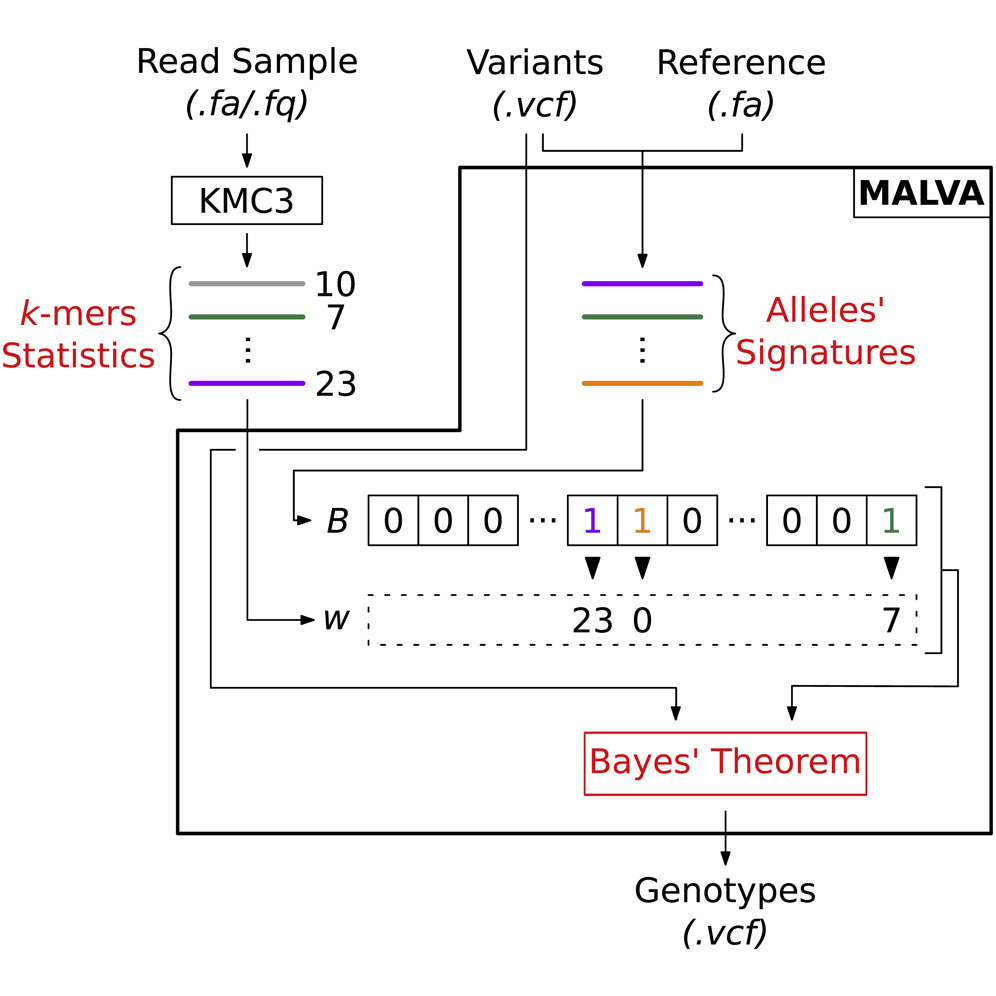
\includegraphics[scale=.90]{images/malva-pipeline.jpg}
  	\caption{Pipeline, MALVA.}
  	\label{fig:malva}
\end{figure}

Il metodo principale è composto da quattro fasi.

Nella prima fase si calcola l'insieme delle firme di lunghezza \textit{${k}_{s}$} di tutti gli alleli alternati di tutte le varianti nel file VCF che vengono memorizzate nell'insieme ALTSIG. Le firme degli alleli di riferimento vengono invece calcolate e memorizzate in un altro set chimato REFSIG. Quindi, vengono memorizzati due pesi per ogni \textit{${k}_{s}$}-mer \textit{t} di una firma: \textit{${w_{t}}_{A}$} rappresenta il numero di occorrenze di \textit{t} nella \textit{signature} di un allele alternato e \textit{${w_{t}}_{R}$} nella \textit{signature} di un allele di riferimento. Nel costruire le firme di un allele bisogna controllare anche tutti gli alleli delle varianti nel raggio di $\lfloor \frac{ {{{k}_{s}} }}{2}  \rfloor$: usando il file VCF vengono ricostruite le sequenze in base alle informazioni sul genotipo che include. 

Nella seconda fase viene effettuato il rilevamento delle \textit{signature} ripetute: per piccoli valori di  \textit{${k}_{s}$} la probabilità che i  \textit{${k}_{s}$}-mer che compongono una firma compaiano in altre regioni del genoma è alta. Poiché successivamente si sfrutteranno le firme degli alleli di ciascuna variante per chiamare i genotipi, la presenza di regioni conservate del genoma di riferimento identiche a una firma potrebbe portare il framework a a genotipizzare erroneamente alcune varianti. Si utilizza perciò il contesto attorno all'allele per distinguere le firme da tali regioni. Se un  \textit{${k}_{s}$}-mer di una firma di un allele alternato appare in qualche parte nel genoma di riferimento, MALVA estrae il contesto di lunghezza  \textit{${k}_{c}$} della regione del genoma di riferimento attorno a tale  \textit{${k}_{s}$}-mer (con  \textit{${k}_{c}$} $>$  \textit{${k}_{s}$}) e raccoglie tali  \textit{${k}_{c}$}-mer in un terzo set, REPCTX. In pratica, si rilevano e memorizzano nel set REPCTX  tutti i  \textit{${k}_{c}$}-mer della sequenza di riferimento il cui \textit{${k}_{s}$}-mer centrale è incluso in alcune \textit{signature} di alleli alternati. 

Nella terza fase MALVA estrae tutti i  \textit{${k}_{c}$}-mer dalla read e il rispettivo numero di occorrenze. Per ogni  \textit{${k}_{c}$}-mer  \textit{${t}_{c}$} che appare \textit{w} volte nel campione, viene estratto il  \textit{${k}_{s}$}-mer  \textit{${t}_{s}$} centrale. Se  \textit{${t}_{s}$} è in REFSIG, ovvero è la firma dell'allele di riferimento di una variante, \textit{${w_{{t}_{s}}}^{R}$} è aumentato di \textit{w}. Se  \textit{${t}_{c}$} non è in REPCTX e  \textit{${t}_{s}$} è in ALTSIG, \textit{${w_{{t}_{s}}}^{A}$} viene aumentato di \textit{w}. Altrimenti, se  \textit{${t}_{c}$} è in REPCTX, \textit{${w_{{t}_{s}}}^{A}$} non viene aggiornato, poichè sebbene il suo \textit{${k}_{s}$}-mer centrale sia uguale ad alcuni \textit{signature}  \textit{${k}_{s}$}-mer di allele alternato, è indistinguibile da un'altra regione del genoma che non copre la variante. Notiamo che quando \textit{${w_{{t}_{s}}}^{A}$} non viene aggiornato, potrebbe esserci la possibilità di non contare una variante del donatore e riportare un falso negativo: per grandi valori di  \textit{${k}_{c}$} ciò accade raramente. Questa è stata una scelta di progettazione: si preferisce evitare bias dovuti ai  \textit{${k}_{c}$}-mer nelle regioni conservate del genoma di riferimento, preferendo non contare l'allele alternato ogni volta che sorgono ambiguità.

Nella quarta e ultima fase MALVA utilizza i pesi delle \textit{signature} calcolati nella fase precedente e le informazioni sugli alleli memorizzate nel file VCF in input per determinare il genotipo di ciascuna variante. Vengono estesi gli approcci proposti in letteratura per le varianti bi-alleliche, in particolare quello introdotto in LAVA \cite{shajii2016lava},) alle varianti multi-alleliche, poichè è necessario calcolare la probabilità dei vari possibili genotipi. Data \textit{v} una variante con (\textit{n} - 1) alleli alternati, il numero di possibili genotipi distinti è $\binom{n}{2} + n = \dfrac{n(n+1)}{2}$, rispettivamente un genotipo di riferimento omozigote, $\binom{n}{2}$ genotipi eterozigoti e (\textit{n} - 1) genotipi alternati omozigoti. MALVA calcola la probabilità di ciascun genotipo utilizzando il teorema di Bayes e il teorema della probabilità assoluta. Viene calcolata la probabilità a priori di ogni genotipo e la probabilità condizionata della \textit{coverage} osservata
dato il genotipo considerato: per computare queste probabilità vengonp nuovamente usate le \textit{signature} e i pesi calcolati nelle fasi precedenti. Dopo aver detrminato la probabilità di ciascun genotipo, MALVA restituisce in output come genotipo predetto quello con la più alta probabilità.



 \textcolor{red}{ secondo te devo aggiungere dettagli implementativi? come il fatto che nel terzo passaggio usa KMC3 per scansionare la read e fare i conteggi in maniera efficiente... questo equivale anche a dire cosa è KMC3.
 }

%Invece di scansionare tutti i kc-mers nella read, MALVA usa KMC3 per estrarli in modo efficiente e contare le loro occorrenze: nel terzo passaggio si analizza l'output di KMC3 e si aggiornano dii conseguenza i conteggi per ogni ks-mer.


\subsubsection{Prestazioni}
 \textcolor{red} {credo questa parte non ci vada, ci sono solo confronti e test con altri tool da mettere alla fine, no singole prestazioni}
 


\end{document}